\chapter{Umsetzung}
\section{Rekonstruktion und Migration der Simulationsumgebung}
Der Quellcode der alten Arbeit liegt auf GitHub\footnote{\url{https://github.com/MobMonRob/HindernisumfahrungRLStudien/tree/1c0a884c2133107562e4928bfa8bef2ee6e2ade0}} vor.
Im ersten Schritt wird angestrebt, diesen Arbeitsstand zu rekonstruieren, sodass ein Training in der Unity-Umgebung möglich ist.

\subsection{Programmversionen}
Zur Projektbasis liegt neben der Ausarbeitung in \cite{waidner.2020} nur Quellcode vor.
Leider werden dabei die verwendeten Programmversionen nicht dokumentiert, welche jedoch notwendigerweise fein aufeinander abgestimmt sein müssen, um ein Training zu ermöglichen und dessen Erfolg zu gewährleisten.
Sowohl Unity als auch ML-Agents und das zugehörige Python-Toolkit wurden seit der Durchführung von \cite{waidner.2020} in unterschiedlicher Geschwindigkeit weiterentwickelt.
Aufgrund von auftretenden Inkompatibilitäten empfiehlt es sich daher, zunächst die ursprünglich verwendeten Versionen aufzusetzen und diese Konstellation als Ausgangspunkt für weitere Anpassungen zu nutzen.
Die Unity-Projektdatei enthält Informationen über die exakte Unity-Version, die zur Erstellung des Projekts verwendet wurde.
Leider fehlt jedoch Dokumentation zur verwendeten Version von ML-Agents und des Python-Toolkits.
Recherche in der Veröffentlichungshistorie von ML-Agents ergibt, dass höchstwahrscheinlich Version 0.14.1 des Unity-Plugins verwendet wurde.
Daraus ergeben sich Python-Abhängigkeiten, die darauf hindeuten, dass eine Python Version \textgreater= 3.6 und \textless 3.7 verwendet wurde.
Leider gestaltet sich der Versuch erfolglos, diese Versionen auf den verwendeten Entwicklungssystemen (OS X und Linux) zu installieren.
Somit ist es auch nicht möglich, die exakte Entwicklungskonstellation von \cite{waidner.2020} zu rekonstruieren.

Um die Ergebnisse dieser Arbeit möglichst nachhaltig zu machen, soll zur weiteren Entwicklung die aktuelle Version von ML-Agents verwendet werden (Unity-Paket in der Version 2.0.1, Stand: Mai 2023).
Das korrespondierende Python-Plugin ist \code{mlagents} in der Version 0.30.0.
(Zum Zeitpunkt des Schreibens ist es notwendig, das Paket \code{protobuf} in der Version 3.20.3 explizit zu installieren, da sonst die Installation von \code{mlagents} scheitert.)
Die Dependencies dieses Pakets bedingen, dass als neuste Python-Version 3.10.8 verwendet werden kann, welche auch zur Entwicklung gewählt wird.

(Die Installation und das Management spezifischer Patch-Versionen von Python kann kompliziert sein, da in der Regel ein Versionsmanagement nur anhand der Minor-Versionen vorgesehen ist.
Im Rahmen dieser Arbeit hat sich der Einsatz des Programms \code{pyenv}\footnote{\url{https://github.com/pyenv/pyenv}} empfohlen, da sich damit sehr einfach spezifische Versionen von Python individuell kompilieren und managen lassen.)

Da es einerseits Problematiken bereiten kann, neue Plugins mit einer alten Version von Unity zu betreiben und zusätzlich die damals verwendete Version massive Fehler in Kombination mit OS X aufweist, wird auch Unity auf eine aktuelle Version angepasst.
Dafür wird in diesem Fall die aktuellste LTS-Version zum Zeitpunkt der Entwicklung verwendet (2021.3.21.f1).

\subsection{Änderungen der Codebasis}
Da es sich bei ML-Agents um ein vergleichsweise neues Toolkit handelt, unterliegt es fortlaufend einer starken Entwicklung.
Im Zeitraum seit der Vorgängerarbeit wurde das Plugin von einer Alphaversion zu einem offiziellen Release gebracht.
In dieser Entwicklungsphase kommt es bei Software häufig zu Breaking Changes.
Auch bei ML-Agents ist dies der Fall und es kommt umgehend zu Kompilierungsfehlern, wenn das Unity-Projekt im Editor geöffnet wird.
Der erste Schritt besteht deshalb darin, herauszufinden, welche Methoden davon betroffen sind.
Dafür werden im Fehlerbericht die Methoden gesucht, die Fehler enthalten.
Die Methodenköpfe können dann in der Versionshistorie von ML-Agents\footnote{\url{https://github.com/Unity-Technologies/ml-agents/releases}} gesucht werden.
Im vorliegenden Fall sind somit alle an der Schnittstelle des Toolkit vorgenommenen Änderungen deutlich aufgeschlüsselt und geben Aufschluss darüber, wie die Kompatibilität des Quellcodes wiederhergestellt werden kann.

Für das Training wird in \cite{waidner.2020} eine Konfiguration in Form einer YAML-Datei verwendet, wie sie in \autoref{sec:training} beschrieben wird.
Mit einer Aktualisierung des Python-Toolkits hat sich auch das Format dieser Datei verändert, weshalb die ursprüngliche Datei nicht mehr kompatibel zum nun verwendeten Tooling ist.
Die Änderungen am Format sind vergleichsweise gering und die Datei von überschaubarer Größe, weshalb nach dem Vorbild der alten Datei und unter Anleitung von \cite{mlagentsHyperparameter} die Datei neu gebaut werden kann.
Der Codestand ist nach diesen Veränderungen\footnote{\url{https://github.com/MobMonRob/HindernisumfahrungRLStudien/tree/ec8abbd161217c9a42adb42779e01c5b3dfeb209}} nun mit den aktualisierten Versionen des Toolings kompatibel und wird als Ausgangspunkt für die Experimente dieser Arbeit verwendet.

\subsection{Durchführung des Trainings}
Um ein Training in der Simulationsumgebung durchzuführen wird zuerst eine kompilierte Binary der Trainingsumgebung erstellt.
Zwar ist es theoretisch möglich, direkt aus dem Unity-Editor das Training zu starten, allerdings bringt dies einige Nachteile mit sich, wie etwa mangelnde Skalierbarkeit und Performanceverluste.
Außerdem ist es so nicht möglich, das Training effizient auf einer unabhängigen Maschine durchzuführen, die eine weit höhere Trainingsrate ermöglicht.
Um eine solche Binary zu erstellen, wird der Build Prozess in Unity unter File \textgreater Build Settings \textgreater Build gestartet.
Dabei wird die gewünschte Zielplattform ausgewählt -- in Abhängigkeit, wo das Training durchgeführt werden soll.
Voraussetzung des Cross-Compiling ist es allerdings, dass die entsprechenden Erweiterungen und Bibliotheken bei der Installation von Unity ausgewählt und geladen wurden.
Andernfalls ist standardmäßig nur das Kompilieren für die Architektur und Plattform möglich, unter der der Editor ausgeführt wird.

Auf der Maschine, auf der das Training durchgeführt wird, muss für die Durchführung des Trainings lediglich das Python-Toolkit installiert sein.
Eine Installation von Unity ist nicht erforderlich, was das Auslagern des Trainingsprozesses und somit ein effizientes Training deutlich vereinfacht.
Für die Experimente im Rahmen dieser Arbeit wird ein virtuelles Rechencluster mit einer Intel Xeon (Gold 6240) CPU mit 8 Kernen, einer Nvidia vGPU V100D-8C und Ubuntu 20.04.1 LTS verwendet.
Deshalb wird das Environment für Linux x86\_64 gebaut und es ist kein Cross-Compiling von der Entwicklungsmaschine zur Trainingsmaschine nötig.

Unity produziert bei Kompilierung für Linux einen Ordner mit den Ausgabedateien, welche sowohl die eigentliche Binary als auch Artefakte und Libraries enthalten.
Dieser Ordner sollte deshalb vollständig auf die Trainingsmaschine übertragen werden.

Für die Durchführung des Trainingsprozesses können verschiedene Parameter der \ac{cli} angepasst werden.
Es ist keine pauschale Angabe möglich, welche Parameter verlässlich und auf allen möglichen Trainingsmaschinen zu einem guten Ergebnis führen.
Deshalb ist eine kleine Testreihe unerlässlich, bei der möglichst gute Werte für die Parameter ermittelt werden, um das spätere Training effizient zu gestalten.
Der maßgebliche Performanceindikator ist hierbei die Anzahl der Trainingsschritte pro Sekunde.
Zur Optimierung wird beispielsweise nach und nach die Anzahl der parallelen Trainingsumgebungen erhöht, bis die Anzahl der Schritte pro Sekunde nicht mehr weiter steigt.
Die nachfolgende Befehlszeile scheint nach einigem Optimieren gute Ergebnisse für die Maschinenkonfiguration zu liefern:
\code{mlagents-learn --env binary-name/binary-name.x86\_64 --run-id runName --no-graphics --torch-device cuda --num-envs 4 --time-scale 1 trainer.yaml}.
Dabei werden 4 parallele Trainingsumgebungen (mit jeweils 30 Agenten) ohne Generierung von grafischen Artefakten betrieben.
ML-Agents greift intern auf TensorFlow und PyTorch zurück.
Grundsätzlich bieten beide Bibliotheken die Möglichkeit, eine CUDA-fähige GPU zur Grafikbeschleunigung der Trainingsalgorithmen zu verwenden.
Im Kontext des verwendeten Trainingsalgorithmus (\ac{ppo}) ist infrage zu stellen, ob ein ernstzunehmender Vorteil durch die Verwendung einer GPU erzielt werden kann.
Ressourcen im Internet sind sich hierüber uneinig.
Da es jedoch nicht zu einer Verschlechterung und bestenfalls zu einer Verbesserung kommen kann, und die GPU zur Verfügung steht, wird sie dem Trainingsprozess auch als Ressource zur Verfügung gestellt.

Weiterhin wird die Wahl getroffen, die \code{time-scale} des Trainingsprozesses auf 1 zu setzen.
Standardmäßig wird dieser Parameter von ML-Agents auf 20 gesetzt, was den Trainingsprozess beschleunigen soll.
Vergleichende Tests ergeben jedoch, dass es im Kontext der verwendeten Trainingsumgebung und Trainingsmaschine keinen Unterschied für die Geschwindigkeit der Trainingsoperationen zu machen scheint, auf welchen Wert der Parameter gesetzt wird.
Es gibt jedoch Hinweise, dass bestimmte Arten von physikalischen Berechnungen von der zeitlichen Skalierung beeinflusst werden \cite{zhang2021}.
Da unklar ist, ob solche Berechnungen hier Verwendung finden und gegebenenfalls sogar eine Ursache für die eigenartige Fortbewegungsart des Roboters im bisherigen Training sein könnten, wird für das Training, wie bereits erwähnt, eine nicht-verzerrte Zeitskala verwendet.
(Da jedoch der Parameter die Schritte pro Sekunde nicht zu beeinflussen scheint, ist zu hinterfragen, ob er in der verwendeten Version der Toolkits überhaupt korrekt interpretiert wird.)

\begin{figure}[H]
    \centering
    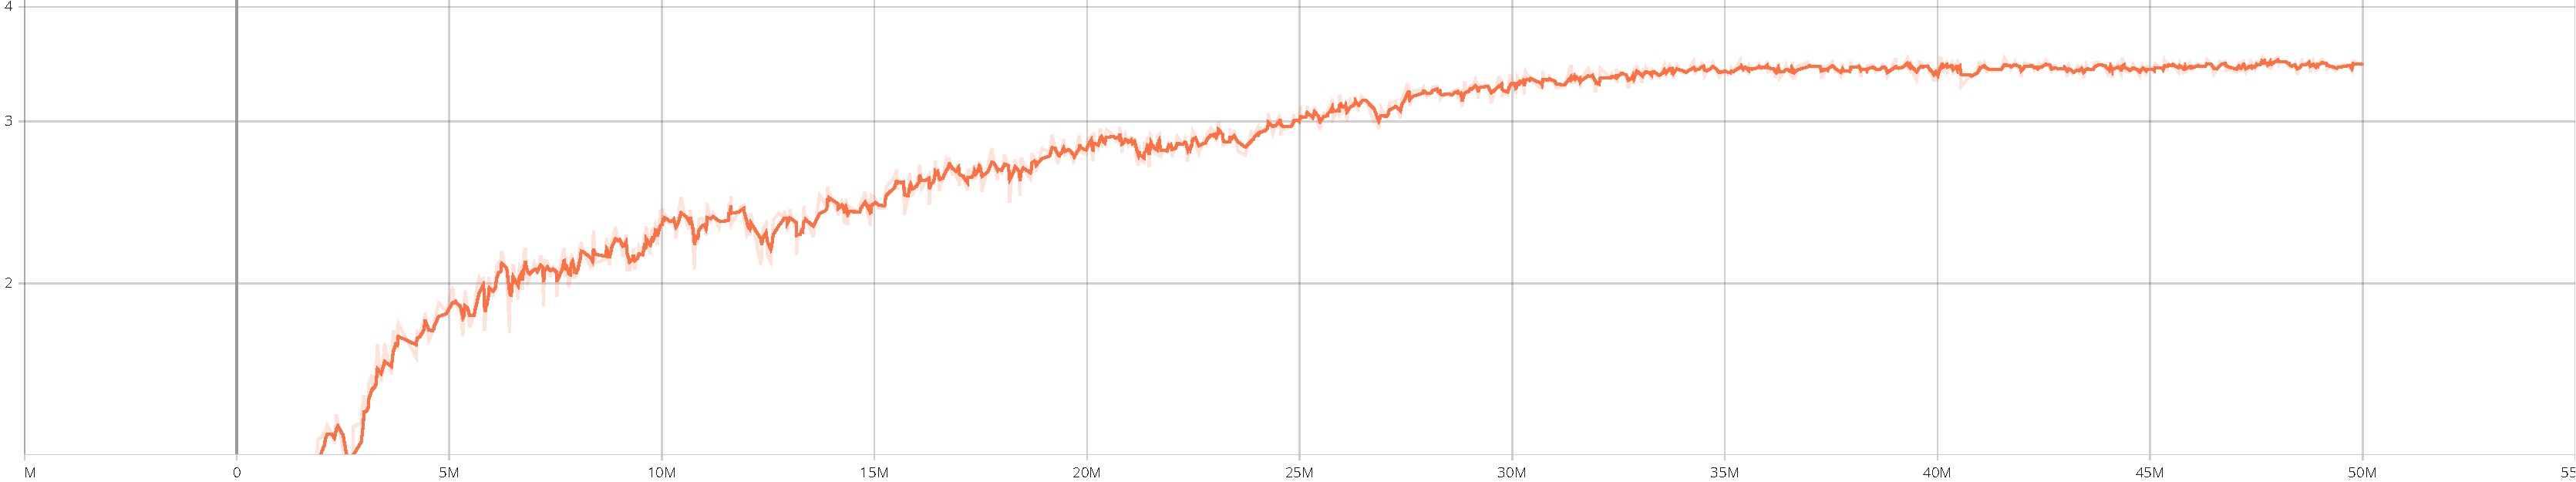
\includegraphics[width=\textwidth]{Bilder/ml-agents/Environment_Cumulative Reward_time-scale-1.pdf}
    \caption{Cumulative Reward der Rekonstruktion von \cite{waidner.2020}}
    \label{fig:time-scale-1}
\end{figure}

Der Verlauf des Cumulative Rewards, der nun beim Training entsteht und in \autoref{fig:time-scale-1} dargestellt wird, gleicht im Wesentlichen den Resultaten von \cite[50]{waidner.2020}.
Auch der gelernte Bewegungsablauf, der bei der Inferenz zu beobachten ist\footnote{\href{https://github.com/yschiebelhut/studienarbeit-doc/raw/master/Videos/SpiderBotDemos/timeScale1.webm}{Link zu Videomaterial}}, gleicht den Resultaten der früheren Arbeit, weshalb die Rekonstruktion als erfolgreich bewertet wird.


\section{Stabilisierung des Laufverhaltens}
Wie in \autoref{sec:probleme} ausgeführt und von den Ergebnissen der Rekonstruktion zusätzlich veranschaulicht wird, bewegt sich der Roboter aktuell mit einer sprungartigen Bewegung fort.
Diese ist, wie beschrieben, Ursache für viele potenzielle Probleme.
Deshalb soll das Laufverhalten stabilisiert werden.
In diesem Zusammenhang wird darunter verstanden, die Schwankungen, die die Körpermitte bei der Bewegung vollführt, auf ein Minimum zu begrenzen.
Wird das Vorbild der Spinnen betrachtet, so ist davon auszugehen, dass diese Einschränkung kein Hindernis für eine effiziente Fortbewegung darstellt.

Innerhalb der Simulation existieren zwei elementare C\#-Skripte, die für die in diesem Kapitel beschriebenen Änderungen von besonderer Relevanz sind: \code{SpiderAgent.cs} und \code{SpiderController.cs}.
In \code{SpiderAgent.cs} befinden sich die für den Reinforcement Learning Prozess relevanten Konfigurationen des Agents.
Dort werden Obsrevations gesammelt und dem Lernalgorithmus zur Verfügung gestellt, die Aktionen vom Lernalgorithmus entgegengenommen, die Lernepisoden verwaltet und vor allem der Reward zugewiesen.
Ein \code{SpiderController} ist wiederum einem \code{SpiderAgent} als Attribut zugeordnet und verwaltet dessen Skripte für die Servomotoren, koordiniert die allgemeine Durchführung der Bewegung und führt das Zurücksetzen der Komponenten durch.
Da ein \code{SpiderController} somit auf die direkten Werte des Roboterzustands zugreifen kann, wird hier auch der Reward berechnet, der in \code{SpiderAgent.cs} zugewiesen wird.

Für die Stabilisierung der Bewegung bestehen zwei verschiedene Ansätze, die ausprobiert und verglichen werden.
Beide werden über Änderungen in \code{SpiderController.cs} realisiert.
Die dort implementierte, allgemeine Bewegungskoordination des Roboters ist eine seiner physikalischen Grundeigenschaften und wird deshalb im Rahmen dieser Arbeit nicht manipuliert.
Auch wird so eine kontinuierliche Basis für die einzelnen Versuche und deren Evaluation geboten.
Jedoch stellt der in dieser Klasse berechnete Reward die zentralste Stellschraube des Reinforcement Learning Problems dar.

\begin{figure}
    \lstinputlisting[
        % language = C,
        firstline = 8,
        % lastline = 41,
        caption = Ürsprüngliche Berechnung des Reward-Signals,
        label = code:reward-post-reconstruct
    ]{Code/post-reconstruct/reward.cs}
\end{figure}

In \autoref{code:reward-post-reconstruct} ist die ursprüngliche Berechnung des Rewards zu sehen, wie sie in \code{SpiderController.cs} implementiert ist.
Dabei wird zunächst der Reward mit 0 initialisiert.
Anschließend wird abgeprüft, ob sich der Roboter um mehr als 90° zur horizontalen Achse gedreht hat und eine negative Belohnung vergeben, falls dies der Fall ist.
Mit dieser Prüfung wird verhindert, dass der Roboter sich überschlägt und dabei seine empfindliche Elektronik beschädigt.
Anschließend wird geprüft, wie weit der Roboter auf der Karte in Vorwärtsrichtung von seinem Ausgangspunkt entfernt ist und die Differenz zum vorherigen Resultat dieser Berechnung gebildet.
Diese Differenz -- sowohl wenn diese positiv ausfällt, als auch, wenn sie negativ ist -- wird dann mit der eventuellen Strafe für ein Überschlagen verrechnet und als Reward zurückgegeben.

Der offensichtliche und einfache Weg ist es nun, in der Methode \code{isTurned()} den Schwellwert der Rückgabe von 90° auf einen kleineren Wert, zum Beispiel 5°, zu reduzieren.
Mit dieser Modifikation wird automatisch ein negativer Summand in den Reward eingebracht, wenn die Schwankung der Körpermitte den nun deutlich geringeren Schwellwert überschreitet.
Das Problem hierbei besteht darin, dass die Methode \code{isTurned()} nicht nur zur Berechnung des Rewards verwendet wird, sondern auch in \code{SpiderAgent.cs} die aktuelle Episode terminiert wird, wenn sich der Roboter auf den Rücken dreht.
Wird die beschriebene Modifikation an dieser Methode vorgenommen, so wird auch eine kleine Schwankung der Körpermitte bereits als Überschlag interpretiert und die laufende Trainingsepisode fälschlicherweise beendet.
Wie sich bei einem Trainingsversuch zeigt, führt dies dazu, dass der Roboter kein Laufverhalten lernen kann, da ihm keine Gelegenheit geboten wird, seinen Fehler zu erkennen, zu erforschen und zu korrigieren.
Für eine möglichst stabile Körpermitte sollte der Rotations-Schwellwert möglichst gering sein.
Jedoch wird bei diesem Ansatz ein Training gegenläufig zum sinkenden Schwellwert praktisch unmöglich.

\begin{figure}
    \lstinputlisting[
        % language = C,
        % firstline = 8,
        lastline = 18,
        caption = Reward-Funktion mit Stabilisierung,
        label = code:reward-1-adjustAngle
    ]{Code/1-adjustAngle/reward.cs}
\end{figure}

Eine alternative Lösung ist in \autoref{code:reward-1-adjustAngle} dargestellt.
Zentrales Element dieser Lösung ist die neu eingeführte Methode \code{getAngle()}.
Der Methodenrumpf ist fast identisch mit dem der Methode \code{isTurned()} aus \autoref{code:reward-post-reconstruct}.
Der Unterschied besteht dabei darin, dass die neue Methode nicht prüft, ob der berechnete Winkel größer als 90° ist und den resultierenden Wahrheitswert zurückgibt, sondern stattdessen den Rest der Division des Winkels durch 90 bestimmt und als Fließkommazahl zurückliefert.
Anschließend wird der mit der neuen Methode berechnete Winkel mit einem kleinen negativen Faktor multipliziert und dieser Summand in der Berechnung des Rewards ergänzt (Zeile 6).
Somit wird eine Strafe vergeben, deren Betrag proportional mit der Rotation der Körpermitte zunimmt.
Die anschließende Belohnung für die zurückgelegte Distanz und die Verrechnung mit der Bestrafung bleibt unverändert.

\begin{figure}
    \centering
    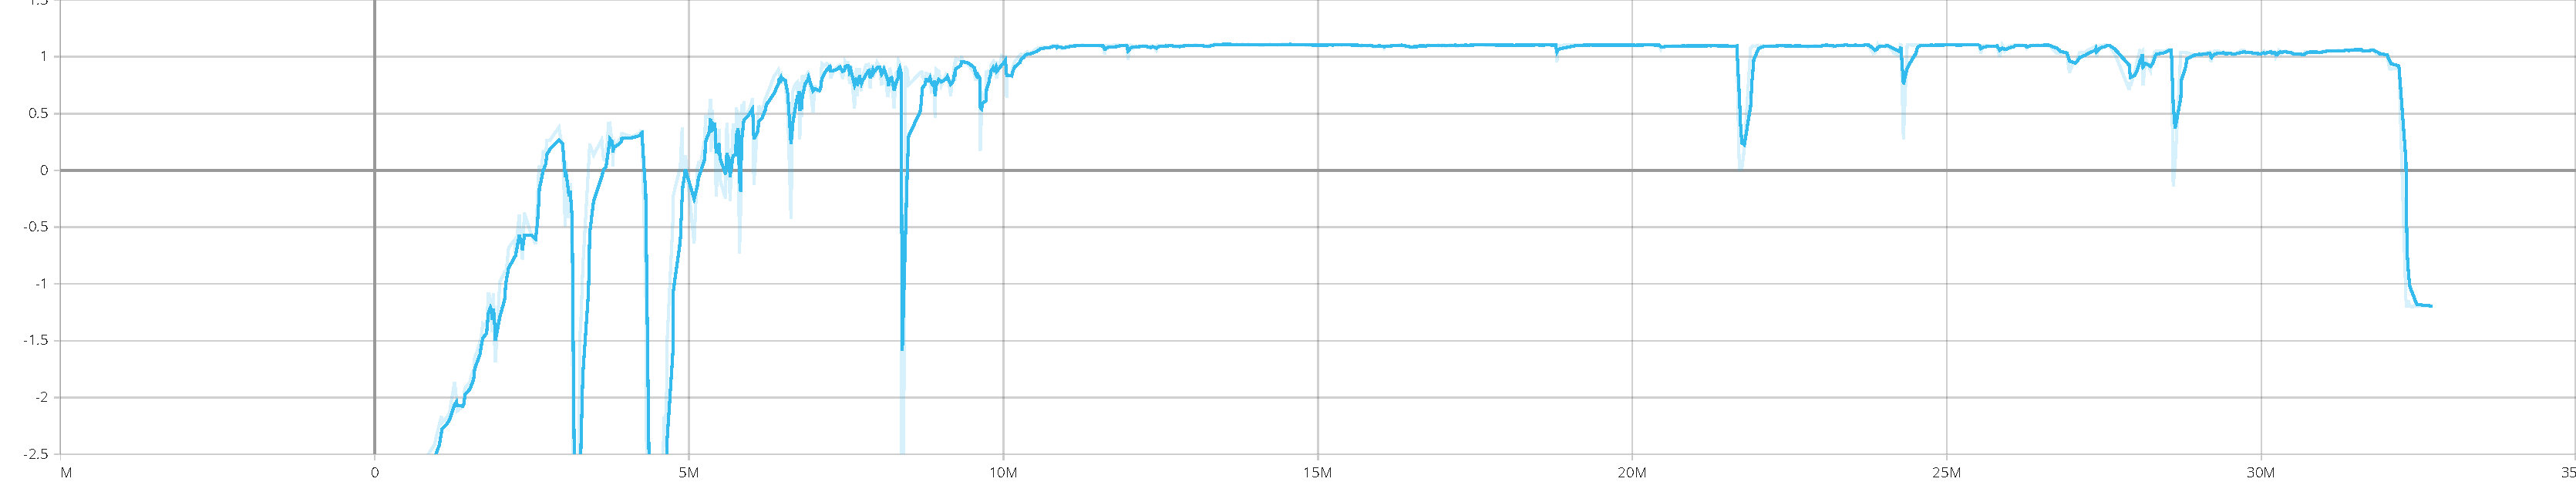
\includegraphics[width=\textwidth]{Bilder/ml-agents/Environment_Cumulative Reward_adjustedAngles.pdf}
    \caption{Cumulative Reward mit Stabilisierung}
    \label{fig:adjustedAngles}
\end{figure}

Das mit dieser Reward-Funktion trainierte Modell legt die Wirksamkeit der Maßnahme dar: beim Laufverhalten des Roboters ist zu beobachten, dass die Körpermitte perfekt in einer horizontalen Lage gehalten wird.
\autoref{fig:adjustedAngles} zeigt den Verlauf des Cumulative Rewards während des Trainings.
Im Vergleich zu \autoref{fig:time-scale-1} fällt auf, dass der Trainingsprozess zwar zu einem stabilen Wert konvergiert, jedoch besonders am Anfang deutlich instabiler verläuft.
Außerdem ist der Wert, zu dem das Training konvergiert, fast um zwei Drittel gemindert.
Betrachtet man das Laufverhalten des Roboters\footnote{\href{https://github.com/yschiebelhut/studienarbeit-doc/raw/master/Videos/SpiderBotDemos/adjustedAngles.webm}{Link zu Videomaterial}}, so fällt weiterhin auf, dass der Roboter weiterhin eine sprungartige Fortbewegung wählt.
(Diese fällt allerdings weitaus stabiler aus, als der in \cite{waidner.2020} erlernte Bewegungsablauf.)
Dabei werden allerdings nur die beiden vorderen und eins der hinteren Beine verwendet, das letzte Bein ist eingekringelt und berührt den Boden nicht.

\subsection{Optimierung der Reward-Funktion}
In einem Versuch, das Laufverhalten weiter zu optimieren und eine natürlichere Laufbewegung zu erhalten, wird die Berechnung des Rewards leicht umgestaltet.
Die optimierte Version ist in \autoref{code:reward-4-no-box} abgebildet.
Die Prüfung, ob der Roboter sich überschlagen hat, bleibt bestehen, wobei hier die Bestrafung erhöht wird, um den Überschlag als schlimmstmöglichen Fall vom instabilen Laufverhalten abzugrenzen.
Tritt dieser Fall ein, so findet auch keine weitere Berechnung des Rewards statt, sondern der Wert der Strafe wird umgehend zurückgegeben.
Danach wird eine kleine Strafe eingeführt, die mit jedem Schritt vergeben wird.
Diese stellt eine generelle Optimierung der Reward-Funktion dar, da eine solche Strafe bewirkt, dass ein Agent danach strebt, sein Ziel möglichst schnell zu erreichen \cite{mlagentsReward}.

Durch die starke Modifikation der Gewichte in der Reward-Funktion können die Beträge der Cumulative Reward Funktion während des Trainings nicht mehr als vergleichende Metrik eingesetzt werden.
Der in \autoref{fig:4-debug} dargestellte Kurvenverlauf zeigt jedoch, dass der Trainingsprozess bedeutend stabiler verläuft verglichen mit \autoref{fig:adjustedAngles}.
Das in Folge der vorgenommenen Maßnahmen trainierte Modell\footnote{\href{https://github.com/yschiebelhut/studienarbeit-doc/raw/master/Videos/SpiderBotDemos/4-debug-extended-vector-size.webm}{Link zu Videomaterial}} zeigt ein erstaunlich natürliches Bewegungsmuster, sehr ähnlich zur Fortbewegung eines Spinnentiers.

\begin{figure}
    \lstinputlisting[
        % language = C,
        % firstline = 8,
        lastline = 12,
        caption = Optimierte Reward-Funktion,
        label = code:reward-4-no-box
    ]{Code/4-no-box/reward.cs}
\end{figure}


\begin{figure}
    \centering
    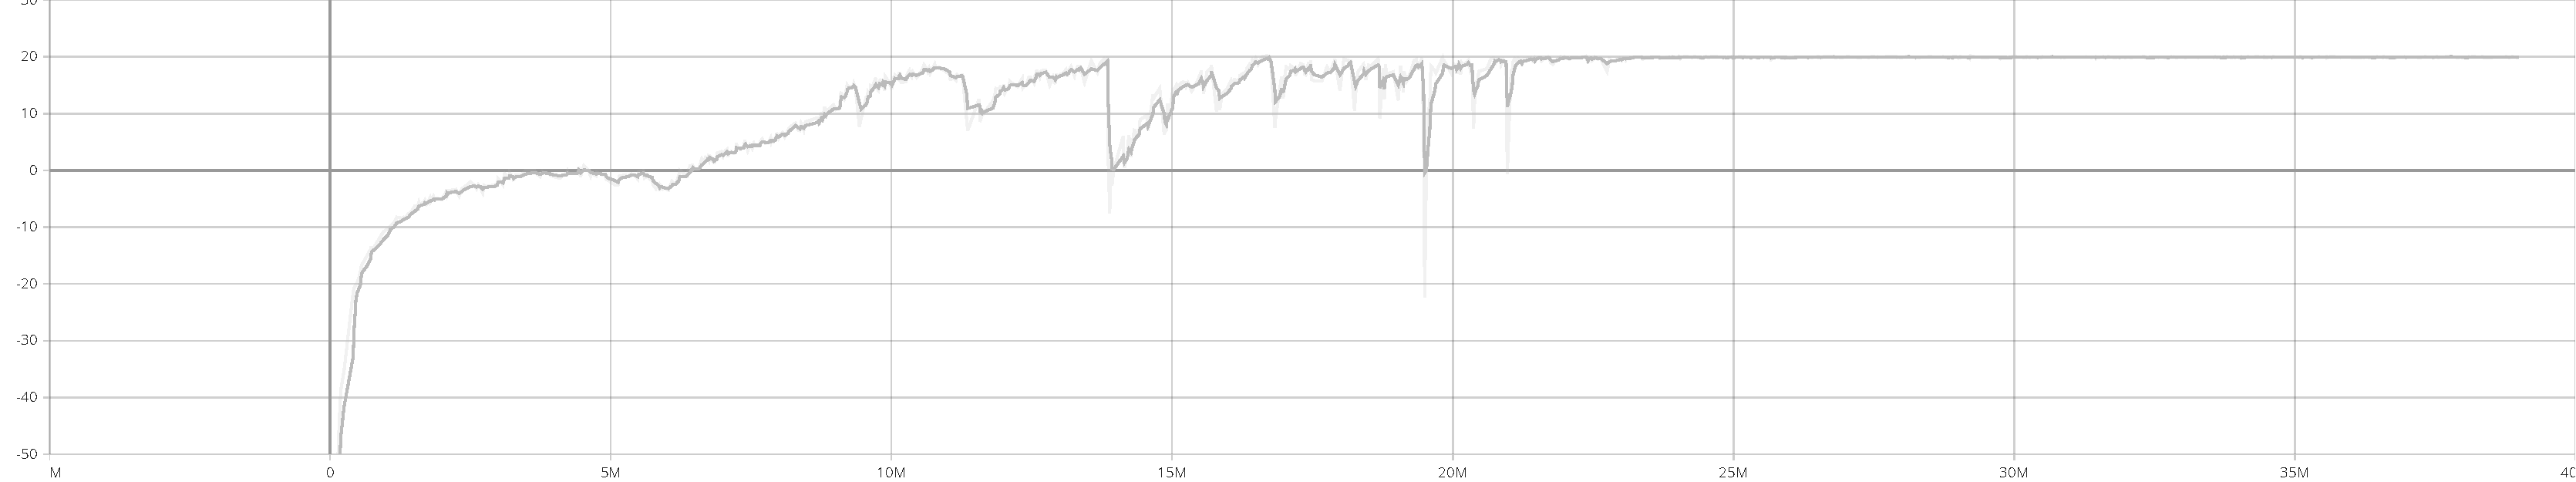
\includegraphics[width=\textwidth]{Bilder/ml-agents/Environment_Cumulative Reward-4-debug-extended-vector-space.pdf}
    \caption{Cumulative Reward mit Optimierung der Reward-Funktion}
    \label{fig:4-debug}
\end{figure}


\section{Pfadplanung}
Der nächste Implementierungsschritt ist die Ergänzung von Pfadplanung.
Hierfür wird zunächst ein Proof of Concept erstellt und dieses im Anschluss auf den Roboter übertragen.

\subsection{Proof of Concept: Crawler}
Wie in \autoref{sec:realisierung} erwähnt, bietet das \emph{Crawler-Example} des ML-Agents-Toolkits eine interessante Referenz für die Pfadplanung.
Im Beispiel wurde ein Agent darauf trainiert, nacheinander zu zufällig erscheinenden Zielen zu laufen.
Wenn der Agent ein Ziel (\emph{DynamicTarget}) erreicht, so verschwindet es und taucht an anderer Stelle wieder auf.
Der Agent hat dabei keinen Einfluss auf das DynamicTarget und kennt nur dessen aktuelle Position.

Wenn ein DynamicTarget initialisiert wird oder in Kontakt mit einem Unity GameObject kommt, welches mit dem Tag \enquote{agent} versehen ist, wird die in \autoref{code:dynamic-target-old} dargestellte Methode ausgeführt, welche das DynamicTarget an einen zufälligen Ort teleportiert.

\begin{figure}
    \lstinputlisting[
        % language = C,
        % firstline = 8,
        % lastline = 12,
        caption = Respawnen des DynamicTargets,
        label = code:dynamic-target-old
    ]{Code/crawler/TargetController-extract.cs}
\end{figure}

Mittels der Modifikation aus \autoref{code:dynamic-target-new} ist es möglich, Einfluss auf die Reihenfolge zu nehmen, in der die DynamicTargets erscheinen.
Die Kontrollstruktur basiert auf einem Zähler und einer Liste von Positionen (Zeile 1f).
Solange der Zähler mit einem Listenindex korrespondiert (Zeile 5), wird als neue Position des Ziels die in der Liste hinterlegte Position verwendet.
Wurde die Liste vollständig abgearbeitet, erscheinen die Ziele wieder zufällig.
In der Element-Detailansicht von Unity können anschließend beliebig viele Zielpunkte frei eingegeben werden (\autoref{fig:eingabefeld-positionen}).

\begin{figure}
    \lstinputlisting[
        % language = C,
        % firstline = 8,
        % lastline = 12,
        caption = Modifiziertes Respawnen des DynamicTargets,
        label = code:dynamic-target-new
    ]{Code/crawler/PathTargetController-extract.cs}
\end{figure}

\begin{figure}
    \centering
    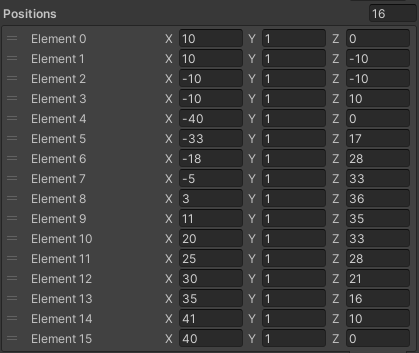
\includegraphics[width = 0.5\textwidth]{Bilder/crawler/position-list.png}
    \caption{Eingabefeld der Positionen}
    \label{fig:eingabefeld-positionen}
\end{figure}

Da der Agent im Crawler-Example die Ziele nicht selbst kontrolliert, ist kein erneutes Trainieren des Modells nötig, sondern die Modifikationen sind direkt wirksam und der Agent läuft entlang des vorgegebenen Pfades\footnote{\href{https://github.com/yschiebelhut/studienarbeit-doc/raw/master/Videos/crawler-poc.webm}{Link zu Videomaterial}}.

\subsection{Übertragung auf den SpiderAgent}
Um dieses Prinzip für den Roboter in dieser Studienarbeit zu nutzen, werden der \code{TargetController} und das dazugehörige Prefab aus dem Beispielprojekt des ML-Agents-Toolkits in die Simulationsumgebung kopiert.
\code{SpiderAgent.cs} wird im Anschluss um den in \autoref{code:dynamic-target-spawn} dargestellten Code ergänzt.
Dieser stellt eine Verknüpfung zwischen dem Agent und dem Target her und ermöglicht das initiale Spawnen des Ziels.
Weiterhin wird sämtlichen Körperteilen des Roboters der Tag \enquote{agent} zugewiesen.
Für das Training wird die Positionsliste leer gelassen, um die Targets zufällig auf der Trainingsplattform erscheinen zu lassen, damit der Roboter nicht einen vorgegebenen Pfad auswendig lernt.


\begin{figure}
    \lstinputlisting[
        % language = C,
        % firstline = 8,
        % lastline = 12,
        caption = Ergänzung für Spawnen des Targets (SpiderAgent.cs),
        label = code:dynamic-target-spawn
    ]{Code/targetAddition.cs}
\end{figure}

Bislang verfügt der Roboter nur über die aktuellen Winkel der Servomotoren als Observations.
Für das weitere Training sollen ihm nun zusätzlich seine eigene Position und die Position des Ziels zugänglich gemacht werden, da es für den Algorithmus andernfalls nicht möglich ist, seine Aktionen auf das Erreichen des Ziels auszurichten.
Alternativ könnte dem Roboter ein Richtungsvektor übergeben werden, der vom Roboter auf das Ziel zeigt.
Hinsichtlich ihres Informationsgehalts sind beide Angaben identisch, da sie rechnerisch ineinander überführt werden können.
Da bei der manuellen Berechnung des Richtungsvektors jedoch leichter Fehler auftreten können, werden absolute Positionen übergeben.
Außerdem wird dadurch zukünftig das Verbinden eines beliebigen Ortungssystems potenziell einfacher gehalten.

Als Voraussetzung, um die zusätzlichen Informationen zur Verfügung zu stellen, muss in Unity die Größe des Observation Space um sechs Elemente erhöht werden, da beide zu übergebenden Positionen jeweils von einem dreidimensionalen Vektor repräsentiert werden.
Anschließend wird die in \autoref{code:observations} dargestellte Methode zum Sammeln der Observations modifiziert.
Vor der Modifikation bestand die Methode lediglich aus der Schleife, die die einzelnen Werte der Servomotoren ausliest und in den VectorSensor eingibt.
Diese Informationen werden um die beiden zusätzlichen Positionen ergänzt.
Die gesamte Anzahl aller Einträge, die in dieser Methode zugewiesen werden muss exakt der in Unity hinterlegten Größe des Observation Space entsprechen, ansonsten erzeugt die Methode Fehler.

\begin{figure}
    \lstinputlisting[
        % language = C,
        % firstline = 8,
        % lastline = 12,
        caption = Erweiterung des Observation Space (SpiderAgent.cs),
        label = code:observations
    ]{Code/extendedVectorSpace/observations.cs}
\end{figure}

\subsection{Geometrische Reward-Funktion}
Um den Roboter nun dazu zu animieren, nicht mehr geradeaus, sondern zu den Zielen zu laufen, wird die Reward-Funktion angepasst.
Wie in \autoref{sec:realisierung} beschrieben, existieren dafür verschiedene Ansätze.
Als der vielversprechendste erscheint dabei die Verwendung einer sogenannten geometrischen Funktion.
Kennzeichnend für diese ist, dass die einzelnen Bestandteile des Rewards nicht wie bislang aufsummiert werden, sondern ein Produkt aller Faktoren gebildet wird.
Damit soll vermieden werden, dass sich der Agent darauf konzentriert, den einfachsten Reward zu maximieren und damit etwa in einem lokalen Maximum stecken zu bleiben.
Um das Produkt zu maximieren, müssen zwangsläufig alle einzelnen Faktoren maximiert werden.

Es werden Trainings für drei solcher Funktionen durchgeführt.
Die Funktionen haben verschiedene Komplexitäten und Ansätze, um eine allgemeine Eignung einer solchen Reward-Funktion abzuschätzen.
\begin{itemize}
    \item Für den ersten Ansatz wird die Distanz gemessen, die der Roboter seit dem letzten Schritt zurückgelegt hat.
    Ausschlaggebend für die Messung ist dabei nur die Körpermitte.
    Als zusätzlicher Faktor wird der Winkel zwischen der \enquote{Blickrichtung} der Körpermitte und der relativen Richtung, in der das Ziel liegt, gebildet und auf einen Bereich von 180° normalisiert.

    \item Die zweite Variation verwendet die in Unity GameObjects hinterlegte Geschwindigkeit der einzelnen Körperteile und bildet daraus den Durchschnitt.
    Dieses Vorgehen soll plötzliche und ruckartige Bewegungen des Roboters, die beim Training auftreten, ausgleichen.
    Der nächste Faktor ist, wie bei der ersten Variante, ein normalisierter Wert an dem abgelesen werden kann, ob die Bewegung in Richtung Ziel erfolgte.
    Weiterhin wird hier wieder eine Belohnung eingeführt, die umso höher ausfällt, desto stabiler die Körpermitte in der Horizontalen gehalten wird.

    \item Der letzte Ansatz ist sehr ähnlich zum zweiten.
    Allerdings wird hier auf das berechnete Produkt noch eine konstante Strafe für jeden Schritt summiert, um eine schnelle Zielerreichung voranzutreiben.
\end{itemize}

Trotz der Unterschiede der Ansätze zeigen alle ein ähnliches Ergebnis des Trainings: der Roboter fällt mit seiner Körpermitte auf den Boden und bewegt seine Beine in der Luft.
Der Cumulative Reward ist dabei relativ konstant, das Modell lernt auch nach mehreren Millionen Simulationsschritten nicht.

\subsection{Klassischer Reward}
\label{sec:classic-reward}
Aus diesen Gründen wird die Entscheidung getroffen, die Reward-Funktion neu zu entwerfen und dabei möglichst wenig konzeptionelle Änderungen ausgehend vom stabilisierten Laufverhalten vorzunehmen.
Ziel dieser Vorgehensweise ist es, die Quellen potenzieller Fehler möglichst weit einzuschränken.
Es wird grundlegend dieselbe optimierte Reward-Funktion wie in \autoref{code:reward-4-no-box} genutzt.
Der Unterschied besteht hierbei jedoch darin, dass nicht mehr die zurückgelegte Distanz entlang der x-Achse gemessen wird, sondern die zurückgelegte Distanz in Richtung des Ziels.
Dafür wird die jeweils letzte Position des Roboters zwischengespeichert.
Es werden dann die Distanzen von der letzten Position zur Zielposition sowie von der aktuellen Position zur Zielposition gebildet.
Anschließend wird die Differenz der beiden Distanzen so bestimmt, dass die Berechnung in einer positiven Belohnung resultiert, wenn der Roboter sich dem Ziel genähert hat.

Dieser Ansatz zeigt bessere Ergebnisse als die mit geometrischer Reward-Funktion, jedoch wird im Training sehr früh ein lokales Maximum erreicht.
Dabei lernt der Roboter, dass er eine Belohnung erzielt, wenn er sich in Richtung des Ziels rollen lässt, überschlägt sich dabei allerdings und startet somit die Trainingsepisode neu.
Versuche, die Strafen für Überschlagen und Körperrotation anzuheben, schlagen ebenfalls fehl.
Wird diese Maßnahme ergriffen, verschlechtern sich die Resultate sogar.
Anstatt sich in Richtung des Ziels zu rollen, rollt sich der Roboter auf dem Boden ein und vollführt nur minimale Bewegungen.

\subsection{Optimierung der Hyperparameter}
Aufgrund der geringen Abweichung der aktuellen Reward-Funktion von \autoref{code:reward-4-no-box} und des simplen Aufbaus der Funktion wird ein Logikfehler in der Funktion als Ursache ausgeschlossen.
Zur Fehlersuche werden erneut Testreihen ausgehend vom Stand des stabilisierten Laufverhaltens durchgeführt und dabei die Änderungsschritte zusätzlich verkleinert.
Dieser letzte Stand enthält als Observationen nur die Winkel der zwölf Servomotoren.
Im ersten Schritt wird nun die Größe des Observation Space erneut, wie oben beschrieben, erweitert.
Dabei werden allerdings nicht die Position des Roboters und die des Ziels hinzugefügt, sondern zwei dreidimensionale Nullvektoren als Platzhalter.
Wie erwartet ist der Cumulative Reward des Trainingsdurchlaufs praktisch deckungsgleich mit dem Stand vor der Veränderung.
Der nächste Schritt fügt nun bei weiterhin gleichbleibender Reward-Funktion die beiden Positionen als Beobachtung anstelle der Nullvektoren hinzu.
Auch wenn zusätzliche Informationen, die allerdings nicht in den Reward einfließen, den Trainingsprozess eigentlich nicht negativ beeinflussen dürften, erreicht der Trainingsprozess mit Zugriff auf die Positionen keinen positiven Cumulative Reward.

Die wahrscheinlichste Ursache für ein solches Verhalten sind suboptimal eingestellte Hyperparameter.
Zusätzlich scheint die Anzahl der Neuronen des verwendeten Neuralen Netzes für die gesteigerte Eingabekomplexität nicht mehr auszureichen.
Aufgrund der Ähnlichkeit des Problems mit dem Crawler-Example, werden die Hyperparameter beider Probleme miteinander abgeglichen und optimiert zusammengeführt.
\autoref{fig:optimierte-hyperparameter} zeigt eine Übersicht der Cumulative Rewards der drei Testläufe.
Die optimierten Hyperparameter werden in \autoref{anhang:trainer-config} dargestellt.

\begin{figure}
    \centering
    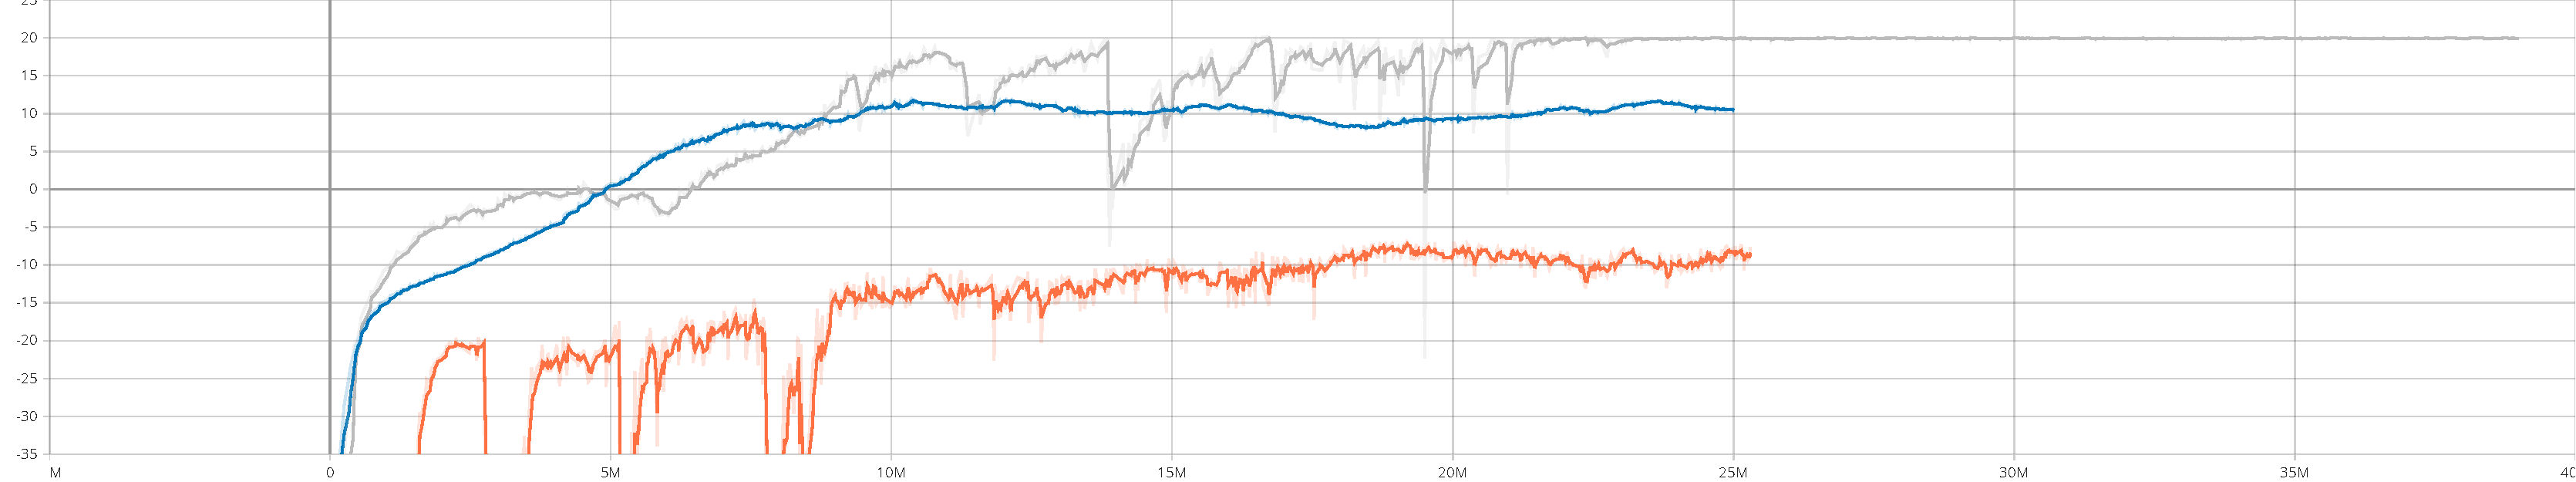
\includegraphics[width = \textwidth]{Bilder/ml-agents/Environment_Cumulative Reward-add-observations.pdf}
    \caption[Schrittweise Erweiterung und Optimierung der Hyperparameter]{Schrittweise Erweiterung und Optimierung der Hyperparameter: (grau) hinzugefügte Nullvektoren; (orange) zusätzliche Beobachtungen bereitgestellt; (blau) optimierte Hyperparameter}
    \label{fig:optimierte-hyperparameter}
\end{figure}

Auf Basis der neu eingestellten Hyperparameter werden erneut die Änderungen von \autoref{sec:classic-reward} angewandt.
Als Resultat kann zwar eine stabil ansteigende Kennkurve des Cumulative Reward beobachtet werden, jedoch trifft dies nicht auf das gelernte Bewegungsverhalten zu.
Der Roboter vollführt eine Mischung aus Sprüngen und Schritten, die ihn teilweise zielstrebig auf das Ziel zubewegen, in anderen Situationen jedoch vollkommen zufällig erscheinen\footnote{\href{https://github.com/yschiebelhut/studienarbeit-doc/raw/master/Videos/SpiderBotDemos/14a-calmed-reward-scaled.webm}{Link zu Videomaterial}}.
In der Dokumentation von ML-Agents wird als Maßnahme für einen stabilen Trainingsprozess empfohlen, den Betrag des Rewards möglichst auf einen Betrag von 1 zu skalieren.
Einige Versuche mit verschiedenen Skalierungen zeigen jedoch keine abweichenden Ergebnisse.
Auffällig ist jedoch, dass die Cumulative Rewards der Trainingsdurchläufe mit skalierten Rewards deutlich stärker schwanken (\autoref{fig:scale-reward}).

\begin{figure}
    \centering
    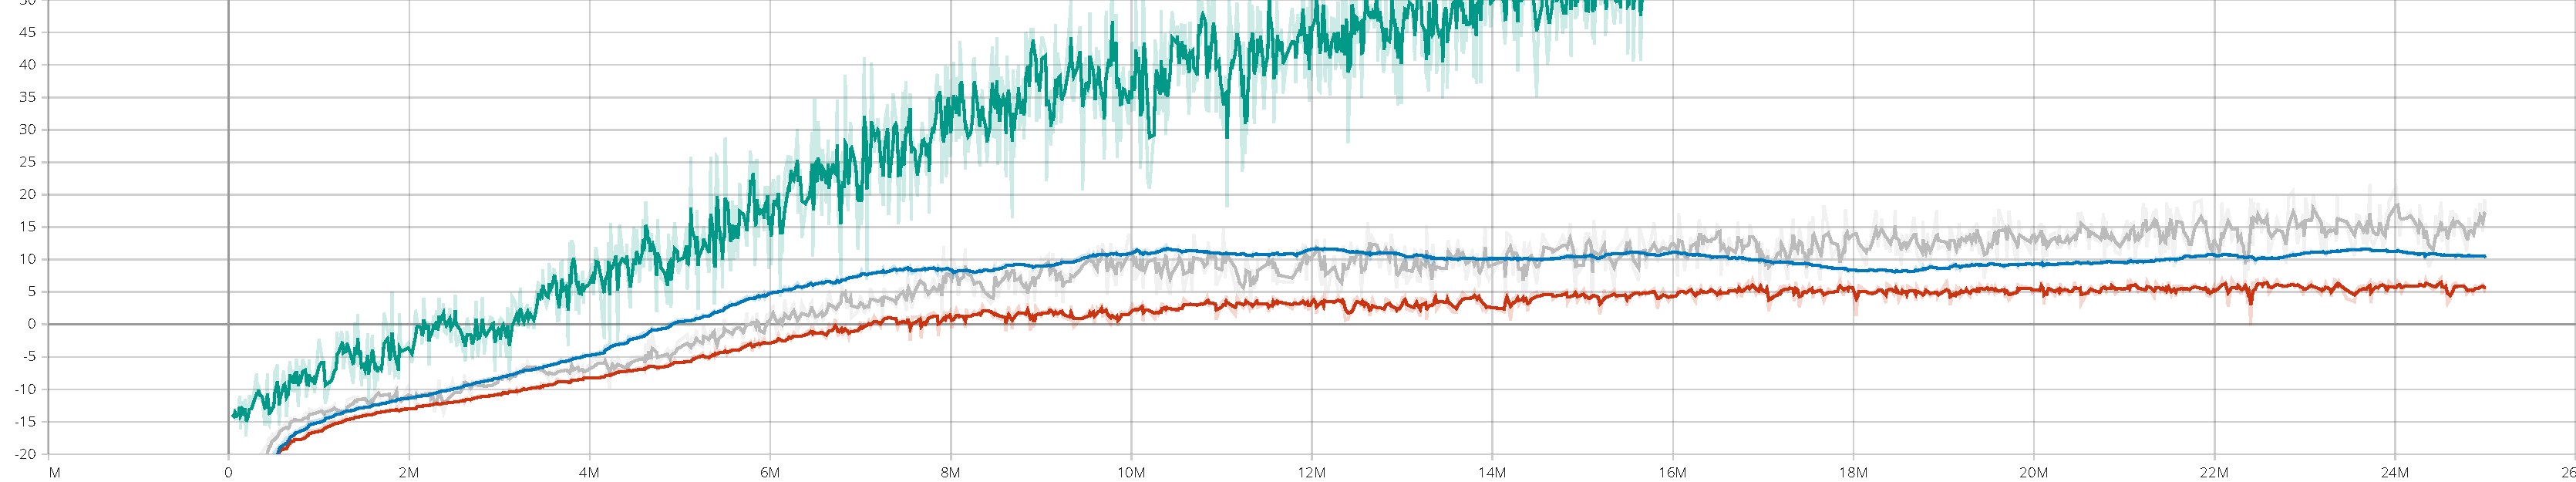
\includegraphics[width = \textwidth]{Bilder/ml-agents/Environment_Cumulative Reward-scale-reward.pdf}
    \caption[Vergleich verschiedener Skalierungen des Rewards]{Vergleich verschiedener Skalierungen des Rewards: (blau) Vergleichskurve geradeaus laufen; (rot) Belohnung für Bewegung in Richtung des Ziels; (grün) skalierter Reward; (grau) skalierter Reward mit höheren Strafen für Schieflage der Körpermitte}
    \label{fig:scale-reward}
\end{figure}

\section{Hindernisumfahrung}
Da Hindernisse nur im Kontext eines vorgesehenen Pfades sinnvoll umsteuert werden können, ist eine funktionierende Pfadplanung eine notwendige Voraussetzung für ein erfolgreiches Training eines Modells, dass den Roboter Hindernisse umsteuern lässt.
Da die im vorherigen Kapitel trainierte Pfadverfolgung keine verwendbare Basis darstellt, werden im Folgenden ein paar grundlegende Aspekte thematisiert und demonstriert.

Um zu sehen, wie der Roboter auf einem einfachen Pfad auf ein statisches Hindernis reagiert, werden ein paar Experimente auf Basis des laufstabilisierten Modells durchgeführt.
Als Pfad ist hier das Laufen entlang der x-Achse zu betrachten, wobei anzumerken ist, dass es keinen Faktor gibt, der eine seitliche Abweichung entlang der z-Achse korrigieren würde.
Stellt man dem normal trainierten Modell ein Hindernis orthogonal zu seiner Laufrichtung in den Weg, so kann man beobachten, dass der Roboter bis an das Hindernis läuft und auch nach der Kollision seine Gangbewegung noch unverändert ausführt, dabei seine Beine allerdings nur auf der Stelle über den Boden schiebt.
Von solch einem Ergebnis ist ohne explizites Training auch auszugehen, da der Roboter nie lernt, zur Seite zu gehen.

Wird nun allerdings mit unveränderter Reward-Funktion und zusätzlich mit dem eingefügten Hindernis trainiert, kann ein interessantes Ergebnis beobachtet werden.
Wie in \autoref{sec:realisierung} schon ausgeführt, lernt der Roboter seine Umgebung auswendig, wenn sich diese nicht verändert.
Dies ist auch hierbei zu beobachten.
Was allerdings verwundert, ist, dass der Roboter schon zu Beginn anfängt, eine Kurve zu laufen, mit der er knapp am Hindernis vorbeikommt -- jedoch wird diese Kurve nicht abgebrochen, wenn der Roboter am Hindernis vorbeilaufen kann, obwohl er dadurch ausschließlich negative Rewards bekommen kann.
Dies widerspricht eigentlich einer der grundlegendsten Maxime von Reinforcement Learning: den Reward immer und um jeden Preis zu maximieren.

Im Falle des Crawler-Examples, anhand dessen ein Proof of Concept zur Pfadplanung implementiert wurde, kann ähnliches beobachtet werden wie bei dem Modell des SpiderAgents, welches nicht explizit für das Hindernis trainiert wurde.
Aufgrund seiner physikalischen Simulationseigenschaften federt der Crawler etwas von der Wand zurück, gegen die er wiederholt läuft.
Dabei wird er jedes Mal leicht zur Seite abgedrängt, wodurch er nach einiger Zeit das Hindernis überwindet.
Dieser Vorgang ist jedoch weder eine gezielte Handlung noch ansatzweise effizient\footnote{\href{https://github.com/yschiebelhut/studienarbeit-doc/raw/master/Videos/crawler-obstacle.webm}{Link zu Videomaterial}}.

Diese Experimente zeigen anschaulich, dass auch bei bereits funktionierender Pfadplanung in jedem Fall ein gesondertes Training mit einem zufällig generierten Hindernisparcours notwendig ist, um dem fertigen Modell ein Umsteuern von Hindernissen zu ermöglichen.
Für den Fall, dass das Erlernen von Pfadplanung und das gleichzeitige Umsteuern von Hindernissen ein zu komplexes Lernproblem darstellt, könnte gegebenenfalls Curriculum Learning eingesetzt werden, um die Probleme aufeinander aufbauend zu lösen.
Insgesamt dürfte eine Hindernisumfahrung langfristig nur sinnvoll sein, wenn sie mit Sensorik unterstützt wird.
Da dies das Problem und dessen Komplexität deutlich verändert, wird dann allerdings ohnehin ein gesondertes Training notwendig sein.